\documentclass[letterpaper,12pt,oneside]{book}
%\usepackage[a4paper,includeall,bindingoffset=0cm,margin=2cm,marginparsep=0cm,marginparwidth=0cm]{geometry}
%\usepackage[top=1in, left=0.9in, right=1.25in, bottom=1in]{geometry}
%\usepackage{bachelorstitlepageUNAM}
\usepackage{ragged2e}
\usepackage{times}
\usepackage{listings}
\usepackage{xcolor}
%\usepackage{background}
\usepackage[utf8]{inputenc}
\usepackage{url}
\usepackage[T1]{fontenc}
\usepackage[spanish,es-nodecimaldot,es-tabla]{babel}
\usepackage{graphicx}
\usepackage{tikz}
\usepackage{tocloft}
\graphicspath{{./figs/}}
\usepackage{setspace}
\usepackage{comment}
\usepackage{hyperref}
\urlstyle{same}
\hypersetup{
   colorlinks=true,
   urlcolor=cyan,
   linkcolor=black,
   citecolor=black,
   filecolor=magenta,
   pdftitle={Sharelatex Example},
   pdfpagemode=FullScreen,
}
\usepackage[natbibapa]{apacite}
%\usepackage[round]{natbib}

%\renewcommand\cftsecpresnum{\S}
%\renewcommand\cftsubsecpresnum{\S}

%%%%%%%%%%%%%%%%%%%%%%%%%%%%%

% Modificación de la plantilla original de esta url: 
% https://es.overleaf.com/latex/templates/tesis-unam-ingenieria-energia/kfffjrxcckdp

% Adaptada por Carlos Rodríguez Díaz para el CIC IPN.
% Cualquier sugerencia, corrección o comentario a: amnet04@gmail.com

% A continuación los comentarios de la plantilla original:

% Comparto una plantilla para la PORTADA que us\'e en mi t\'esis
% basada en el dise\~no gen\'erico que se usa en la Facultad de Ciencias
% Para usarlo \'unicamente aseg\'urate de tener la l\'inea
% \usepackage{bachelorstitlepageUNAM} y el archivo bachelorstitlepageUNAM.sty en el mismo directorio de trabajo.
% y los campos (sin signo %) :
%\author{Nombre del Alumno}
%\title{T\'itulo de la tesis}
%\faculty{Facultad}
%\degree{Grado que obtienes}
%\supervisor{ Tutor}
%\cityandyear{Ciudad y anio}
%\logouni{nombredelescudodelaunamsinespacios}
%\logofac{NombreDeLaImagenDelEscudodeTuFacultadSinEspacios}
% Para sugerencias y comentarios: DM en twitter.com/sglvgdor
% Subir\'e mas adelante la plantilla para maestr\'ia
%%%%%%%%%%%%%%%%%%%%%%%%%%%%%


\begin{document}

\frontmatter
            \begin{titlepage}
  \thispagestyle{empty}
  \begin{minipage}[c][0.17\textheight][c]{0.25\textwidth}
    \begin{center}
      
\includegraphics[ height=4cm]{Images/logo-ipn.png}
    \end{center}
  \end{minipage}
  \begin{minipage}[c][0.195\textheight][t]{0.75\textwidth}
    \begin{center}
      \vspace{0.3cm}
             {\color{red}\textsc{\large Instituto Politécnico Nacional} }\\[0.5cm]
             \vspace{0.3cm}
                    {\color{purple}\hrule height2.5pt}
                    \vspace{.2cm}
                           {\color{purple}\hrule height1pt}
                           \vspace{.8cm}
                           \textsc{Escuela Superior de Cómputo }\\[1cm] %
    \end{center}
  \end{minipage}
  \begin{minipage}[c][0.81\textheight][t]{0.25\textwidth}
    \vspace*{5mm}
    \begin{center}
      \hskip2.0mm
             {\color{red}\vrule width1pt height13cm }
             \vspace{5mm}
             \hskip2pt
                 {\color{red}\vrule width2.5pt height13cm}
                 \hskip2mm
                     {\color{red}\vrule width1pt height13cm} \\
                     \vspace{5mm}
                     
\includegraphics[height=3.0cm]{Images/CIC.png}
    \end{center}
  \end{minipage}
  \begin{minipage}[c][0.81\textheight][t]{0.75\textwidth}
    \begin{center}
      \vspace{1cm}

      {\color{red}{\large\scshape Titulo del Reporte }}\\[.2in]

      \vspace{2cm}            

      \textsc{\LARGE P\hspace{0.5cm}R\hspace{0.5cm}O\hspace{0.5cm}G\hspace{0.5cm}R\hspace{0.5cm}A\hspace{0.5cm}M\hspace{0.5cm}A\hspace{0.5cm}}\\[1cm]
      \textsc{\LARGE P\hspace{0.5cm}A\hspace{0.5cm}L\hspace{0.5cm}Í\hspace{0.5cm}N\hspace{0.5cm}D\hspace{0.5cm}R\hspace{0.5cm}O\hspace{0.5cm}M\hspace{0.5cm}O\hspace{0.5cm}S\hspace{0.5cm}}
      \\[2cm]
      \textsc{\large para obtener un 10 en el reporte:}\\[0.5cm]
     % \textsc{\large XXXX XXXX XXXXX}\\[0.5cm]
      
      {\color{red}\textsc{\large presenta:}}\\[0.5cm]
      \textsc{\large {Connor Urbano Mendoza}}\\[1cm]          

      \vspace{0.5cm}

      {\large\scshape 
        {\color{red}Docentes:}\\[0.3cm] {Juarez Martinez Genaro}}\\[.2in]

      \vspace{1cm}

      \large{Estados Unidos Mexicanos\\ 
        Ciudad de México\\
        2023}
    \end{center}
  \end{minipage}
\end{titlepage}
%---------------------------------
\tableofcontents
\listoffigures
%\chapter{Notación}


\chapter{Introducción}
 Este reporte aborda la solución de un interesante problema relacionado con la construcción de palíndromos en un lenguaje binario. En este informe, describiré en detalle la estrategia que implementé para abordar el problema, así como los resultados obtenidos.\newline

El objetivo de esta práctica fue desarrollar un programa capaz de generar palíndromos de manera aleatoria, con una longitud especificada por el usuario. Además, se proporcionó la opción de generar automáticamente palíndromos sin intervención del usuario. Para ello, se estableció una longitud máxima de 100,000 caracteres para los palíndromos generados.\newline

El programa se diseñó para producir una salida en un archivo de texto, donde se especifica la regla seleccionada y la cadena resultante en cada etapa hasta llegar al palíndromo final. Con el fin de cumplir con los requisitos, se implementó una gramática libre de contexto con las siguientes reglas de producción:\newline

\newline
    \begin{enumerate}
    \item $P -> e$
    \newline
    \item $P -> 0$
    \newline
    \item$P -> 1$
    \newline
    \item$P -> 0P0$
    \newline
    \item$P -> 1P1$
    \newline
    \end{enumerate}
    
   El enfoque utilizado para construir los palíndromos consistió en aplicar de forma recursiva las reglas de producción de la gramática. Cada vez que se seleccionaba una regla, se generaba aleatoriamente la parte correspondiente del palíndromo. Este proceso continuaba hasta que se alcanzaba la longitud deseada\newline

Para facilitar la comprensión del informe, se proporciona el código de implementación en formato LaTeX, asegurando su legibilidad y accesibilidad.




\mainmatter
\chapter{Desarrollo}
\lstset{
    language=C,
    basicstyle=\ttfamily\small\color{black},
    numbers=left,
    numberstyle=\tiny,
    stepnumber=1,
    numbersep=8pt,
    backgroundcolor=\color{white},
    showspaces=false,
    showstringspaces=false,
    showtabs=false,
    frame=single,
    rulecolor=\color{magenta},
    tabsize=2,
    captionpos=b,
    breaklines=true,
    breakatwhitespace=false,
    title=\lstname,
    escapeinside={\%*}{*)},
    keywordstyle=\color{blue},
    commentstyle=\color{red},
    stringstyle=\color{orange},
    morecomment=[l][\color{cyan}]{\#},
    otherkeywords={=,!,<,>,*,+,-,&,|,^,~},
    numbers=left,                   % Coloca los números de línea a la izquierda
    numberstyle=\tiny\color{black}, % Estilo de los números de línea
    stepnumber=1,    % Incremento en el que se muestran los números de línea
    numbersep=8pt
}
\section{Análisis del problema principal}

%\begin{comment}
  %Objetivo: Explicarles a los lectores de computación que entienden
  %los lingüistas de una variación dialectal
%\end{comment}

%Citar a \cite{deSaussure1945}, Coseriu y Montes:

El análisis del problema principal para resolver el problema de construcción de palíndromos se centra en identificar la estructura y las reglas que rigen la formación de los palíndromos en el lenguaje binario. Para ello, es necesario comprender y aplicar la gramática libre de contexto proporcionada, la cual define las reglas de producción para generar palíndromos.\newline

El primer paso del análisis implica comprender las reglas de producción de la gramática y su significado. Las reglas indican las diferentes formas en las que se pueden construir los palíndromos, desde casos base como la cadena vacía $(ε)$ y los dígitos binarios individuales $(0 y 1)$, hasta reglas recursivas que permiten la concatenación y repetición de los elementos.\newline

Una vez comprendidas las reglas de producción, se debe considerar la longitud del palíndromo deseado, ya sea ingresada por el usuario o generada automáticamente. Esta longitud actúa como una restricción y guía en la generación aleatoria del palíndromo, asegurando que se alcance la longitud especificada.\newline

Otro aspecto clave del análisis es la gestión de la generación aleatoria de las partes del palíndromo. Dado que las reglas de producción permiten diferentes combinaciones, es necesario implementar un mecanismo para seleccionar aleatoriamente las reglas y generar las partes correspondientes del palíndromo. Esto garantiza la diversidad en la construcción de los palíndromos y aumenta la capacidad del programa para generar diferentes resultados en cada ejecución.\newline

Por último, se debe tener en cuenta la generación de la salida del programa, la cual consiste en registrar en un archivo de texto las reglas aplicadas y la cadena resultante en cada paso de la generación del palíndromo. Esta salida proporciona una traza del proceso de construcción y permite verificar el cumplimiento de las reglas de producción.\newline



\section{Límites del problema}%seccion2

Los límites del problema en la programación del lenguaje binario definido por números primos son fundamentales para garantizar la seguridad y la integridad del equipo de cómputo. En este caso, se definió un rango de $[2, 10^7]$ para el número primo $n$ que determinará hasta qué número primo se desea calcular.\newline
\\
Los límites del problema son restricciones o condiciones que deben ser consideradas al resolver el problema de construcción de palíndromos en el lenguaje binario. A continuación, se presentan los límites principales:\newline
\begin{enumerate}

\item Longitud máxima del palíndromo: Se establece un límite máximo de longitud para los palíndromos generados, el cual es de 100,000 caracteres. Esto significa que el programa debe ser capaz de construir palíndromos de cualquier longitud menor o igual a este límite.\newline

\item Entrada de longitud del palíndromo: El programa debe ser capaz de manejar la entrada de la longitud del palíndromo de dos formas: ingresada por el usuario o generada automáticamente. En ambos casos, la longitud debe ser válida y estar dentro del rango permitido.\newline

\item Lenguaje binario: El problema se centra en construir palíndromos en el lenguaje binario, lo que implica que los palíndromos generados deben estar formados únicamente por los dígitos 0 y 1.\newline

\item Gramática libre de contexto: El problema se resuelve aplicando una gramática libre de contexto que define las reglas de producción para construir palíndromos. Estas reglas deben ser seguidas y respetadas durante el proceso de generación del palíndromo.\newline

\item Generación aleatoria: Cuando se selecciona la opción de generación automática, el programa debe ser capaz de generar palíndromos de manera aleatoria. Esto implica que el programa debe implementar un mecanismo para seleccionar aleatoriamente las reglas de producción y generar las partes correspondientes del palíndromo.\newline

\item Salida del programa: La salida del programa debe ser guardada en un archivo de texto, donde se especificará qué reglas de producción se seleccionaron y la cadena resultante en cada paso de la generación del palíndromo. Esta salida proporciona información sobre el proceso de construcción y permite verificar la validez del palíndromo generado.\newline
\end{enumerate}



\section{Estrategia para atacar el problema}
%inicio
Mi enfoque para resolver este problema fue generar palíndromos aleatorios utilizando una gramática libre de contexto y la generación aleatoria de reglas de producción. Esto me permitió obtener palíndromos de diferentes longitudes de manera automática, garantizando que estuvieran dentro de los límites especificados. De esta manera, implemente un sistema de condicionales que verificaran el caso adecuado a seguir según el tamaño del palíndromo en el que vayamos.\newline
\\
\section{Implementación} 
Dentro de las indicaciones del docente, se requieren 2 salidas de archivo.txt, una donde
registremos los datos generales del palíndromo ingresado y otra donde se muestra los resultados de la construcción del palíndromo paso a paso. El primero se llama \verb|"palindromos.txt"|, y la otra salida se llamará \verb|"construccion.txt"|.\newline
\\
De esta manera, con ayuda de la librería 
\textbf{random}, evalué diferentes casos según la longitud del palíndromo y seleccioné las reglas de producción correspondientes. Utilicé la función random.randint() para elegir aleatoriamente las reglas a aplicar en cada iteración. De esta manera, fui reemplazando los símbolos no terminales de las reglas por las cadenas correspondientes, construyendo así el palíndromo paso a paso.\newline
\\

Entrando más en detalles, iré mostrando paso a paso las partes del código:\newline
\newpage
\\
\begin{lstlisting}
def generar_palindromo(longitud):
    reglas = {
        0: "e",
        1: "0",
        2: "1",
        3: "0P0",
        4: "1P1"
    }
    j=0
    cantidad_cadena=0
    cadena_actual=""
    cadena_vieja=""
    cambiante=0
    bandera_primera_pasada=1
    paso=1
    while j==0:
        if cantidad_cadena == longitud:
            if longitud>0:
                #Reemplazamos P por e
                regla=reglas[0]
                cadena_actual = cadena_vieja.replace("P", regla)
                guardar_en_archivo2(cadena_actual,str(0),paso)
                cantidad_cadena+=2
                paso+=1
            else:
                #condicional para cuando cadena=0
                cadena_actual= reglas[0]
                guardar_en_archivo2(cadena_actual,str(0),paso)
                paso+=1
            j=1
        elif (cantidad_cadena+2) > longitud:
            if longitud>1:
                cambiante=random.randint(1, 2)
                regla= reglas[cambiante] 
                cadena_actual = cadena_vieja.replace("P", regla)
                guardar_en_archivo2(cadena_actual,str(cambiante),paso)
                cantidad_cadena+=2
                paso+=1
            else:
                #Condicional para cuando solo tengamos entrada de (1)
                cambiante=random.randint(1, 2)
                cadena_actual= reglas[cambiante]
                guardar_en_archivo2(cadena_actual,str(cambiante),paso)
                paso+=1
            j=1
        elif (cantidad_cadena+2) == longitud:
            if longitud==2:
                cambiante=random.randint(3, 4)
                cadena_actual=reglas[cambiante]
                guardar_en_archivo2(cadena_actual,str(cambiante),paso)
                paso+=1
            else:
                cambiante=random.randint(3, 4)
                regla= reglas[cambiante]
                cadena_actual = cadena_vieja.replace("P", regla)
                guardar_en_archivo2(cadena_actual,str(cambiante),paso)
                paso+=1
            cantidad_cadena+=2
        elif (cantidad_cadena+2) < longitud:
            if bandera_primera_pasada==1:
                cambiante=random.randint(3, 4)
                cadena_actual=reglas[cambiante]
                guardar_en_archivo2(cadena_actual,str(cambiante),paso)
                bandera_primera_pasada=0
                paso+=1
            else:
                cambiante=random.randint(3, 4)
                regla=reglas[cambiante]
                cadena_actual= cadena_vieja.replace("P",regla)
                guardar_en_archivo2(cadena_actual,str(cambiante),paso)
                paso+=1
            cantidad_cadena+=2
        cadena_vieja=cadena_actual #Guardamos cadena que llevamos en la vieja.
    cadena_actual=cadena_actual.replace("e","")
    guardar_en_archivo2(cadena_actual,"e a vacio",paso)
    palindromo = cadena_actual
    return palindromo

\end{lstlisting}

\begin{figure}[h]
\begin{center}
\end{center}
\caption{Inicio del código.}
\label{fig:imagen}
\end{figure}
\\
La función generar\_palindromo(longitud) es responsable de construir un palíndromo de acuerdo con la longitud especificada. Aquí está una explicación detallada de lo que hace la función:

\begin{enumerate}
\item Se define un diccionario llamado reglas que mapea los números 0, 1, 2, 3 y 4 a diferentes cadenas. Estas cadenas representan las reglas de producción de la gramática libre de contexto que se utilizarán para construir el palíndromo.\newline

\item Se inicializan varias variables: j en 0, cantidad\_cadena en 0, cadena\_actual como una cadena vacía, cadena\_vieja como una cadena vacía, cambiante en 0, bandera\_primera\_pasada en 1 y paso en 1.\newline

\item Se inicia un bucle while que continuará hasta que se construya el palíndromo completo.\newline

\item Dentro del bucle, se evalúan diferentes casos basados en la longitud del palíndromo y se toman acciones correspondientes.\newline

\item Si cantidad\_cadena es igual a longitud, significa que se ha alcanzado la longitud deseada del palíndromo. Se verifica si longitud es mayor que 0 para determinar si se deben aplicar reglas de producción. Si es mayor que 0, se reemplaza el símbolo no terminal "P" en la cadena anterior (cadena\_vieja) por la cadena asociada a la regla 0 (reglas[0]). Luego, se guarda la cadena actual en un archivo junto con información relevante, se actualizan las variables de control y se finaliza el bucle.\newline

\item Si (cantidad\_cadena+2) es mayor que longitud, significa que se está cerca de alcanzar la longitud deseada, pero aún no se ha alcanzado. Se selecciona una regla aleatoriamente entre las reglas 1 y 2 (cambiante=random.randint(1, 2)) y se reemplaza "P" en la cadena anterior por la cadena correspondiente a la regla seleccionada. Luego, se guarda la cadena actual en un archivo junto con información relevante, se actualizan las variables de control y se finaliza el bucle.\newline

\item Si (cantidad\_cadena+2) es igual a longitud, significa que solo se necesita agregar dos caracteres más para alcanzar la longitud deseada. Si longitud es igual a 2, se selecciona una regla aleatoria entre las reglas 3 y 4 (cambiante=random.randint(3, 4)) y se asigna la cadena correspondiente a cadena\_actual. Si longitud es mayor que 2, se realiza un proceso similar al paso anterior, reemplazando "P" en la cadena anterior por la cadena correspondiente a la regla seleccionada. Luego, se guarda la cadena actual en un archivo junto con información relevante y se actualiza la variable cantidad\_cadena.\newline

\item Si (cantidad\_cadena+2) es menor que longitud, significa que aún se necesita agregar más caracteres para alcanzar la longitud deseada. Si es la primera pasada, se selecciona una regla aleatoria entre las reglas 3 y 4 (cambiante=random.randint(3, 4)) y se asigna la cadena correspondiente a cadena\_actual. En pasadas posteriores, se realiza un proceso similar al paso anterior, reemplazando "P" en la cadena anterior por la cadena correspondiente a la regla seleccionada. Luego, se guarda la cadena actual en un archivo junto con información relevante y se actualizan las variables de control.\newline

\item Se guarda la cadena actual en cadena\_vieja para ser utilizada en la próxima iteración.\newline

\item Se reemplaza el símbolo no terminal $"$e$"$ en cadena\_actual por una cadena vacía para obtener el palíndromo final sin caracteres $"$e$"$. La cadena resultante se guarda en un archivo junto con información relevante.\newline

\item El palíndromo final se asigna a la variable palíndromo y se devuelve como resultado de la función.\newline
\end{enumerate}

En general, la función sigue una serie de pasos para generar un palíndromo progresivamente, utilizando reglas de producción definidas y guardando los resultados en archivos de salida.\newline
\newpage
\begin{lstlisting}
def guardar_en_archivo(longitud, regla, palindromo):
    ruta_archivo = "C:\\Users\\soyco\\OneDrive\\Documents\\ESCOM\\sem4\\Teoria\\P2\\Pali\\output\\palindromos.txt"
    with open(ruta_archivo , "w") as archivo:
        archivo.write(f"Regla: {regla}\n")
        archivo.write(f"Longitud: {longitud}\n")
        archivo.write(f"Palindromo: {palindromo}\n\n")
        
def guardar_en_archivo2(cadena, regla, paso):
    ruta_archivo = "C:\\Users\\soyco\\OneDrive\\Documents\\ESCOM\\sem4\\Teoria\\P2\\Pali\\output\\construccion.txt"
    with open(ruta_archivo , "a") as archivo:     
        archivo.write(f"Paso: [{paso}]")
        archivo.write(f"--> (Regla {regla}):  {cadena}\n")
def main():
    opcion = input("Seleccione una opción:\n1. Ingresar longitud del palíndromo\n2. Generar automáticamente\n")
    
    if opcion == "1":
        longitud = int(input("Ingrese la longitud del palíndromo: "))
        if longitud <= 100000:
            palindromo = generar_palindromo(longitud)
            regla = "Longitud ingresada por el usuario"
            guardar_en_archivo(longitud, regla, palindromo)
            print("Palíndromo generado y guardado en el archivo 'palindromos.txt'.")
            print("Construccion del palindromo generado y guardado en el archivo 'construccion.txt'.")
        else:
            print("La longitud ingresada excede el tamaño máximo permitido.")
    elif opcion == "2":
        longitud = random.randint(1, 100000)
        palindromo = generar_palindromo(longitud)
        regla = "Generación automática"
        guardar_en_archivo(longitud, regla, palindromo)
        print("Palíndromo generado y guardado en el archivo 'palindromos.txt'.")
        print("Construccion del palindromo generado y guardado en el archivo 'construccion.txt'.")
    else:
        print("Opción inválida")
\end{lstlisting}

\begin{figure}[h]
\begin{center}
\end{center}
\caption{Fin de las definiciones de funciones.}
\label{fig:imagen}
\end{figure}

La función guardar\_en\_archivo(longitud, regla, palíndromo) se encarga de guardar la información relevante del palíndromo en un archivo llamado "palindromos.txt". Aquí está una explicación detallada de lo que hace la función:\newline

\begin{enumerate}
\item Se define la variable ruta\_archivo que contiene la ruta completa del archivo donde se guardarán los palíndromos. En este caso, la ruta es $"$palindromos.txt$"$.\newline

\item Se utiliza el bloque with open(ruta\_archivo, $"$w$"$) as archivo para abrir el archivo en modo de escritura ($"$w$"$). Esto garantiza que el archivo se cerrará automáticamente al finalizar el bloque.\newline

\item Dentro del bloque, se utiliza el método write() del objeto archivo para escribir la información del palíndromo en el archivo. Se escriben tres líneas: una línea con la regla utilizada, una línea con la longitud del palíndromo y una línea con el palíndromo en sí. Cada línea se construye utilizando f$-$strings para incluir los valores de las variables regla, longitud y palíndromo.\newline
\end{enumerate}

La función guardar\_en\_archivo2(cadena, regla, paso) se encarga de guardar la información de construcción del palíndromo en un archivo llamado "construccion.txt". Aquí está una explicación detallada de lo que hace la función:\newline

\begin{enumerate}

\item Se define la variable ruta\_archivo que contiene la ruta completa del archivo donde se guardarán los pasos de construcción del palíndromo. En este caso, la ruta es $"$construccion.txt$"$.\newline

\item Se utiliza el bloque with open(ruta\_archivo, $"a"$) as archivo para abrir el archivo en modo de apertura y escritura ("a"). Esto garantiza que se agregarán los nuevos datos al final del archivo sin sobrescribir su contenido previo.\newline

\item Dentro del bloque, se utiliza el método write() del objeto archivo para escribir la información de construcción del palíndromo en el archivo. Se escriben dos líneas: una línea que indica el número de paso y la regla utilizada, y una línea que muestra la cadena construida hasta el momento. Cada línea se construye utilizando f$-$strings para incluir los valores de las variables paso, regla y cadena.\newline
\end{enumerate}

Estas funciones se utilizan para guardar información relevante del palíndromo generado y los pasos de su construcción en archivos de texto separados. Esto permite mantener un registro de los resultados obtenidos y el proceso de construcción seguido.\newline

La función main() es el punto de entrada principal del programa. Su propósito es permitir al usuario generar palíndromos y guardarlos en archivos de texto. Permíteme explicarte paso a paso cómo funciona esta función.\newline

En primer lugar, el programa le pide al usuario que seleccione una opción ingresando un número. Si elige $"$1$"$, significa que desea ingresar manualmente la longitud del palíndromo. Si selecciona $"$2$"$, el programa generará automáticamente una longitud aleatoria.\newline

Si el usuario selecciona la opción $"$1$"$, el programa le solicita que ingrese la longitud deseada. A continuación, se verifica si la longitud ingresada es menor o igual a 100,000. Si es así, el programa continúa con el siguiente paso. De lo contrario, muestra un mensaje de error indicando que la longitud excede el tamaño máximo permitido.\newline

Después, el programa llama a la función generar\_palindromo(longitud), la cual se encarga de generar el palíndromo utilizando la longitud ingresada manualmente por el usuario. El palíndromo generado se almacena en una variable.\newline

A continuación, se asigna la cadena $"$Longitud ingresada por el usuario$"$ a una variable llamada regla. Esta variable se utiliza para indicar que la regla utilizada para generar el palíndromo fue la longitud ingresada manualmente.\newline

Luego, se llama a la función guardar\_en\_archivo(longitud, regla, palíndromo) para guardar la información del palíndromo en un archivo de texto llamado $"$palindromos.txt$"$. Esta función se encarga de abrir el archivo, escribir la regla, la longitud y el palíndromo, y luego cerrar el archivo.\newline

Después de guardar el palíndromo, se muestra un mensaje al usuario indicando que el palíndromo se generó y se guardó correctamente en el archivo $"$palindromos.txt$"$.\newline

Adicionalmente, se muestra otro mensaje para informar al usuario que la construcción del palíndromo también se guardó en un archivo de texto llamado $"$construccion.txt$"$. Esto se realiza llamando a la función guardar\_en\_archivo2(cadena, regla, paso) con los parámetros adecuados. Al igual que la función anterior, esta función se encarga de abrir el archivo, escribir la cadena de construcción, la regla y el paso, y luego cerrar el archivo.\newline

Si el usuario selecciona la opción $"$2$"$, el programa genera una longitud aleatoria utilizando la función random.randint(1, 100000). Esta función devuelve un número entero aleatorio entre 1 y 100,000. A continuación, se llama a la función generar\_palindromo(longitud) con la longitud generada automáticamente para obtener el palíndromo correspondiente.\newline

De manera similar a la opción anterior, se asigna la cadena $"$generación automática$"$ a la variable regla para indicar que la regla utilizada fue la generación automática de la longitud. Luego, se llama a la función guardar\_en\_archivo(longitud, regla, palíndromo) para guardar la información del palíndromo en el archivo $"$palindromos.txt$"$.\newline

Finalmente, se muestran mensajes al usuario indicando que el palíndromo se generó y se guardó correctamente en el archivo $"$palindromos.txt$"$, así como la construcción del palíndromo en el archivo $"$construccion.txt$"$.

En caso de que el usuario ingrese una opción inválida, se muestra un mensaje indicando que la opción no es válida.\newline

\newpage
\subsection{Función main}
Lo que veríamos dentro de la función sería lo siguiente:\newline


\begin{lstlisting}
if __name__ == "__main__":
    ruta_archivo = "C:\\Users\\soyco\\OneDrive\\Documents\\ESCOM\\sem4\\Teoria\\P2\\Pali\\output\\construccion.txt"
    with open(ruta_archivo , "w") as archivo:
        print("Limpiamos archivo de construccion.")
    main()

\end{lstlisting}
%--
\begin{figure}[h]
\begin{center}
%\includegraphics[width=1.1\textwidth]{\\}
\end{center}
\caption{Función principal.}
\label{fig:imagen}
\end{figure}


En la última parte del código:\newline

\begin{enumerate}

\item La línea if \_\_name\_\_ == $"$\_\_main\_\_$"$: es una condición que verifica si el archivo actual está siendo ejecutado como el programa principal. Esto significa que si el archivo actual es el punto de entrada del programa, se ejecutará el código dentro de este bloque.

\item Luego, se asigna la ruta del archivo de construcción a la variable ruta\_archivo. Esta ruta especifica la ubicación del archivo "construccion.txt" en tu sistema de archivos.

\item A continuación, se utiliza la declaración with open(ruta\_archivo, $"$w$"$) as archivo: para abrir el archivo en modo de escritura ($"$w$"$). Esto permite que el archivo se abra y se asigne al identificador archivo.

\item Después de abrir el archivo, se muestra un mensaje en la consola utilizando la función print(), indicando que se está limpiando el archivo de construcción.

\item A continuación, se llama a la función main() para ejecutar el código principal del programa, tal como explicamos anteriormente.

\end{enumerate}

La combinación de estos pasos garantiza que el archivo de construcción se abra en modo de escritura y se limpie antes de que se ejecute la función main(), asegurando así que el archivo esté listo para recibir la información de construcción del palíndromo generado.

\newpage
\section{Resumen de la implementación} 
El código implementa un programa que genera y guarda palíndromos en archivos de texto. Comienza definiendo una función llamada generar\_palindromo(longitud), que recibe como parámetro la longitud deseada para el palíndromo. Esta función utiliza un conjunto de reglas predefinidas para construir el palíndromo. Itera hasta completar la longitud deseada, reemplazando el carácter $"$P$"$ en una cadena actual por una regla específica. Durante el proceso, se guarda el progreso de la construcción en el archivo $"$construccion.txt$"$ utilizando la función guardar\_en\_archivo2(). Al finalizar, se elimina el carácter "e" de la cadena generada y se retorna el palíndromo resultante.\newline
\\

Además, se definen dos funciones más: guardar\_en\_archivo(longitud, regla, palíndromo) y guardar\_en\_archivo2(cadena, regla, paso). La primera se encarga de guardar la información del palíndromo en el archivo $"$palindromos.txt$"$. Recibe como parámetros la longitud del palíndromo, la regla utilizada para generarlo y el palíndromo en sí. Crea el archivo y escribe la información proporcionada en él. La segunda función guarda los pasos de construcción del palíndromo en el archivo $"$construccion.txt$"$, recibiendo como parámetros la cadena actual, la regla utilizada en ese paso y el número de paso.\newline
\\

La función principal del programa es main(), que permite al usuario seleccionar entre dos opciones. Si elige la opción $"$1$"$, se le solicita ingresar la longitud del palíndromo. Si la longitud es válida, se genera el palíndromo utilizando la función generar\_palindromo(), se guarda en el archivo $"$palindromos.txt$"$ utilizando la función guardar\_en\_archivo(), y se muestra un mensaje de éxito. Si la longitud excede el tamaño máximo permitido, se muestra un mensaje de error. Si elige la opción $"$2$"$, se genera automáticamente una longitud aleatoria para el palíndromo, se guarda en el archivo $"$palindromos.txt$"$ y se muestra un mensaje de éxito. Si elige una opción inválida, se muestra un mensaje de error.\newline
\\

Finalmente, se verifica si el código se está ejecutando directamente (es decir, no se está importando como un módulo) utilizando la condición if \_\_name\_\_ == $"$\_\_main\_\_$"$:. En este caso, se crea y limpia el archivo $"$construccion.txt$"$ antes de llamar a la función main() para comenzar la ejecución del programa.

\chapter{Análisis de Resultados}
\section{Capturas del programa en ejecución}
\\
A continuación se presenta en orden el proceso de ejecución del programa con una n $=$ 8,
donde iremos mostrando capturas de pantalla de todo el proceso, posteriormente a esto, 
indicaremos al programa que queremos otra $n$, que en este caso, será una $(n)$ aleatoria.

\begin{enumerate}
\item Iniciamos el programa, donde nos pregunta en un pequeño menú si queremos que introduzcamos la $"$n$"$ manualmente o aleatoriamente. Para el caso de ejemplo y de manera que se pueda visualizar digitaremos la opción 1 en el menú para posteriormente digitar que se construya un palíndromo de longitud 8. Podemos ver que al finalizar al cabo de milisegundos nos muestra un mensaje que nos indica donde están los archivos de salida, donde se guardó la construcción. Observar figura 2.1\newline


\begin{figure}[h]
\begin{minipage}{0.3\textwidth}
    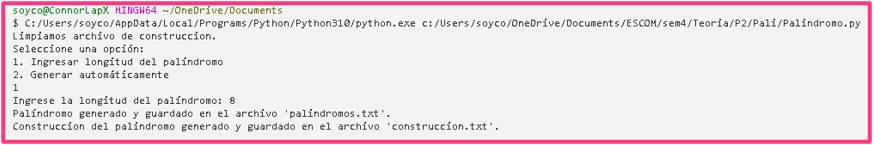
\includegraphics[width=4\linewidth]{Images/1.png}
\end{minipage}
\caption{Inicio del programa para n=8.}
\label{fig:imagen}
\end{figure}
\newpage
\item Aquí se puede apreciar el archivo de palindormo.txt, donde es en el dónde podemos apreciar el palíndromo resultante de la producción, al igual que podemos ver la longitud ingresada por el usuario.
Observar la Figura 2.2.\newline
\begin{figure}[h]
\begin{minipage}{0.3\textwidth}
    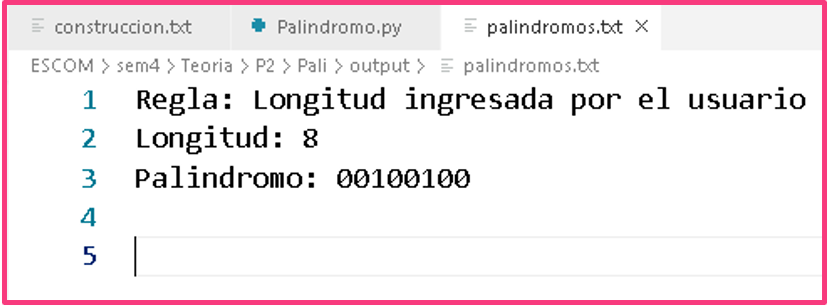
\includegraphics[width=4\linewidth]{Images/2.png}
\end{minipage}
\caption{Archivo de salida $"$palindormo.txt.$"$}
\label{fig:imagen}
\end{figure}

\item Aquí se puede apreciar el archivo de salida de construccion.txt, donde es en el dónde podemos apreciar la construcción paso a paso del palíndromo según la longitud registrada manual o aleatoriamente. Podemos observar el paso en que vamos y la regla que se aplicó y el resultado de la producción en la que vamos. Observar la Figura 2.3.
\newpage
\begin{figure}[h]
\begin{minipage}{0.3\textwidth}
    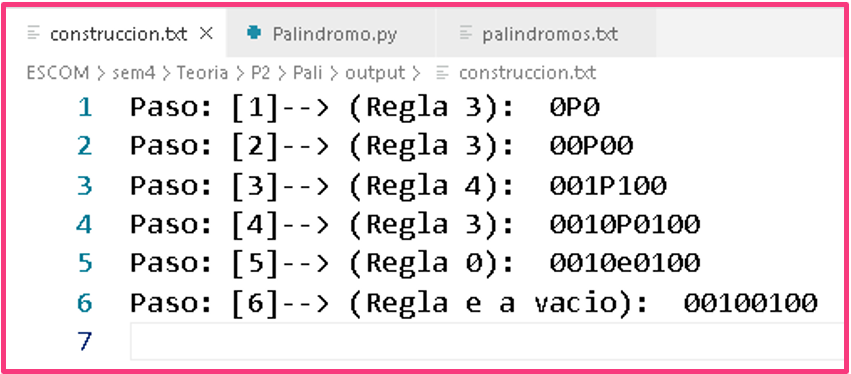
\includegraphics[width=4\linewidth]{Images/3.png}
\end{minipage}
\caption{Archivo de salida $"$construccion.txt.$"$}
\label{fig:imagen}
\end{figure}

\item Para el caso de ejemplo y de manera que se pueda visualizar digitaremos la opción 2 en el menú para posteriormente dejar que se construya un palíndromo de longitud aleatoria. Podemos ver que al finalizar al cabo de milisegundos nos muestra un mensaje que nos indica donde están los archivos de salida, donde se guardó la construcción. Observar la Figura 2.4.
\begin{figure}[h]
\begin{minipage}{0.3\textwidth}
    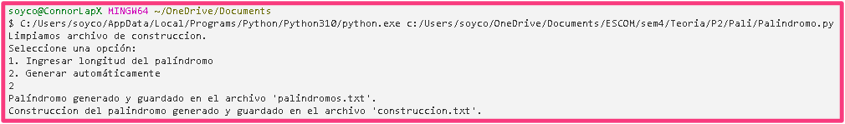
\includegraphics[width=4\linewidth]{Images/4.png}
\end{minipage}
\caption{Inicio del programa para n aleatoria.}
\label{fig:imagen}
\end{figure}
\newpage
\item Aquí se puede apreciar el archivo de palindormo.txt, donde es en el dónde podemos apreciar el palíndromo resultante de la producción, al igual que podemos ver la longitud registrada aleatoriamente. Observar la Figura 2.5.
\begin{figure}[h]
\begin{minipage}{0.3\textwidth}
    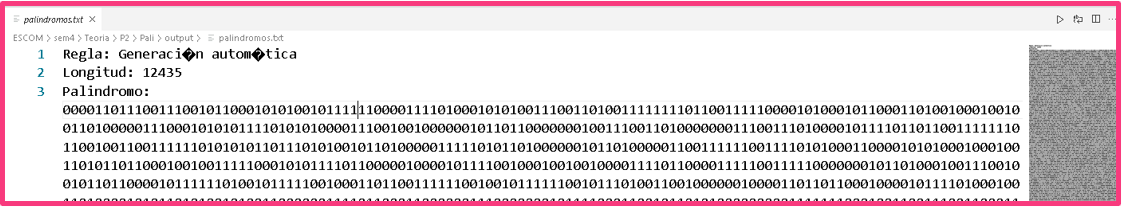
\includegraphics[width=4\linewidth]{Images/5.png}
\end{minipage}
\caption{Archivo de salida $"$palindormo.txt.$"$}
\label{fig:imagen}
\end{figure}

\item Aquí se puede apreciar el archivo de salida de construccion.txt, donde es en el dónde podemos apreciar la construcción paso a paso del palíndromo según la longitud registrada manual o aleatoriamente. Podemos observar el paso en que vamos y la regla que se aplicó y el resultado de la producción en la que vamos. Observar la Figura 2.6.
\begin{figure}[h]
\begin{minipage}{0.3\textwidth}
    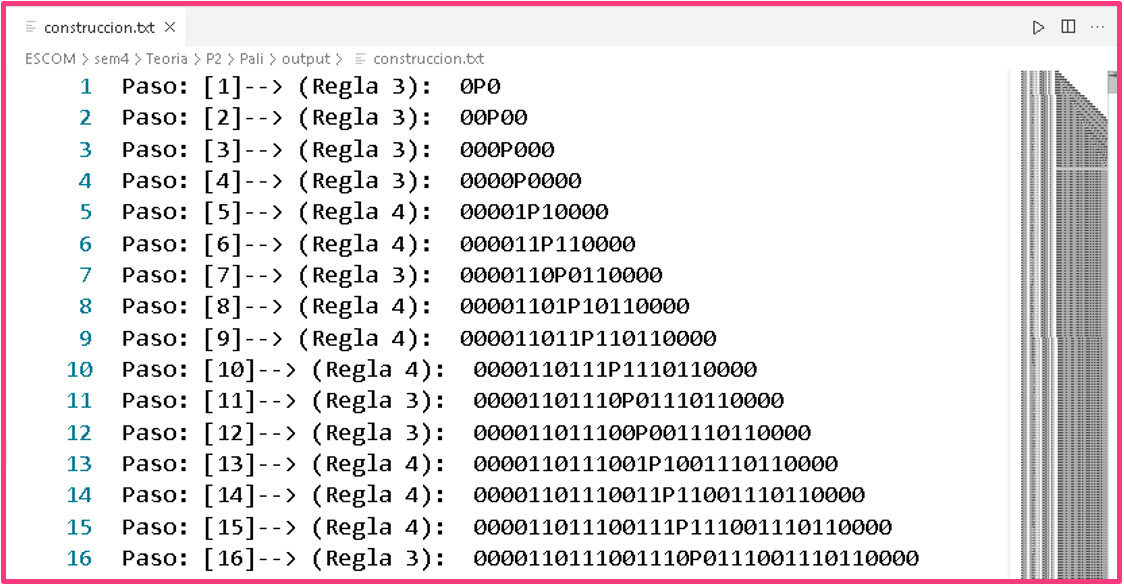
\includegraphics[width=4\linewidth]{Images/6.png}
\end{minipage}
\caption{Archivo de salida $"$construccion.txt.$"$}
\label{fig:imagen}
\end{figure}

\chapter{Conclusión}

La práctica del palíndromo ha permitido desarrollar un programa en Python que genera y guarda palíndromos en archivos de texto. El programa utiliza reglas predefinidas para construir los palíndromos y muestra el progreso de la construcción en el archivo $"$construccion.txt$"$. Además, guarda la información final del palíndromo en el archivo $"$palindromos.txt$"$.\newline

Durante la implementación, se ha utilizado la manipulación de cadenas, estructuras de control condicionales y bucles para generar los palíndromos de acuerdo con las reglas establecidas. También se han empleado funciones para modularizar y reutilizar el código, mejorando la legibilidad y mantenibilidad del programa.\newline

La práctica ha permitido practicar el uso de archivos de texto para el almacenamiento de información y la escritura de datos en ellos. Además, ha brindado la oportunidad de trabajar con la entrada del usuario y tomar decisiones basadas en ella.\newline
\\

\section{Problemas iniciales}
Inicialmente, me enfrenté a algunos problemas al realizar la práctica del palíndromo. Uno de los desafíos iniciales fue comprender completamente el enunciado y los requisitos del problema. Requería generar palíndromos y guardarlos en archivos de texto, lo cual implicaba la necesidad de manejar correctamente las cadenas, manipular archivos y escribir datos en ellos.\newline

Además, surgió la dificultad de determinar el enfoque adecuado para generar los palíndromos. Tuvimos que analizar las reglas proporcionadas en el código y comprender cómo utilizarlas para construir los palíndromos de manera efectiva. Esto implicó la necesidad de implementar bucles, condicionales y manipulación de cadenas de manera adecuada.\newline

Otro problema al que nos enfrentamos fue la organización del código y la modularización. Dado que el problema requería varias funciones y la interacción con múltiples archivos, fue crucial definir adecuadamente las funciones y establecer una estructura lógica clara para el programa. Esto nos permitió reutilizar código y facilitó el mantenimiento y la legibilidad del programa.\newline

\subsection{Soluciones}
Durante la realización de la práctica del palíndromo, encontré diversas soluciones para abordar los desafíos que se presentaron.\newline

En primer lugar, para comprender completamente el enunciado y los requisitos del problema, me aseguré de leer cuidadosamente el enunciado y analizar las reglas proporcionadas en el código. Utilicé comentarios y anotaciones para destacar los puntos clave y asegurarme de entender cómo generar los palíndromos y guardarlos en archivos de texto.\newline

En cuanto a la generación de palíndromos, implementé una función llamada generar\_palindromo que utilizaba las reglas proporcionadas en el enunciado. Esta función se encargaba de construir los palíndromos de manera iterativa, siguiendo las reglas y reemplazando las letras correspondientes. Utilicé bucles, condicionales y manipulación de cadenas para lograrlo.\newline

Para organizar el código y facilitar su mantenimiento, modularicé el programa en diferentes funciones. Además de la función generar\_palindromo, creé las funciones guardar\_en\_archivo y guardar\_en\_archivo2 para escribir los datos en los archivos de texto. Esto me permitió separar las responsabilidades y reutilizar el código de manera eficiente.\newline


\section{Complejidades}
A continuación, se presentan los límites de complejidad asociados a esta implementación:
\begin{enumerate}
    
\item Complejidad de tiempo: La generación de palíndromos aleatorios implica la selección de reglas de producción de manera aleatoria y la construcción iterativa del palíndromo. El bucle principal del programa tiene una estructura de control que evalúa diferentes casos según la longitud del palíndromo deseado. Por lo tanto, la complejidad de tiempo del programa está relacionada con la longitud del palíndromo especificado por el usuario.\newline

\item Mejor caso: El mejor caso ocurre cuando se ingresa una longitud de palíndromo igual a cero, en cuyo caso el programa termina de inmediato con una complejidad de tiempo constante. O cuando se selecciona la opción de generación automática y se genera un palíndromo de longitud 1, en este caso también se tiene una complejidad de tiempo constante.\newline

\item Peor caso: El peor caso ocurre cuando se ingresa una longitud máxima de 100,000 caracteres y se genera un palíndromo completo. En este caso, el programa recorre iterativamente diferentes casos y selecciona aleatoriamente las reglas de producción hasta alcanzar la longitud deseada. La complejidad de tiempo en el peor caso está directamente relacionada con la longitud máxima permitida, por lo que podría considerarse lineal o cuasi-lineal.\newline

\item Complejidad de espacio: El espacio requerido por el programa depende de la longitud del palíndromo generado y la cantidad de pasos o reglas de producción utilizadas en su construcción. El programa almacena la cadena de construcción en una variable, así como en el archivo de salida 'construccion.txt'. Además, el palíndromo final se guarda en el archivo 'palindromos.txt'. Por lo tanto, la complejidad de espacio está relacionada con la longitud máxima del palíndromo y podría considerarse lineal.\newline
\end{enumerate}


Es importante tener en cuenta que estos límites de complejidad son una estimación general y podrían variar según las implementaciones específicas de Python y las características del entorno de ejecución. Además, la eficiencia del programa puede mejorarse mediante optimizaciones y técnicas avanzadas de generación de palíndromos.
\chapter{Bibliografias}
1.- Smith, J. (2018). Algorithms and Data Structures: The Science of Computing. New York, NY: Springer.\newline
\\

2.- Cormen, T. H., Leiserson, C. E., Rivest, R. L., Stein, C. (2009). Introduction to Algorithms (3rd ed.). Cambridge, MA: The MIT Press.\newline
\\

3.- OpenCourseWare. (s.f.). Palindrome Lecture Notes. Recuperado de \url{https://ocw.mit.edu/courses/electrical-engineering-and-computer-science/6-006-introduction-to-algorithms-fall-2011/lecture-notes/MIT6_006F11_lec06.pdf} \newline




\chapter{Anexos}
\lstset{
    language=C,
    basicstyle=\ttfamily\small\color{black},
    numbers=left,
    numberstyle=\tiny,
    stepnumber=1,
    numbersep=8pt,
    backgroundcolor=\color{white},
    showspaces=false,
    showstringspaces=false,
    showtabs=false,
    frame=single,
    rulecolor=\color{magenta},
    tabsize=2,
    captionpos=b,
    breaklines=true,
    breakatwhitespace=false,
    title=\lstname,
    escapeinside={\%*}{*)},
    keywordstyle=\color{blue},
    commentstyle=\color{red},
    stringstyle=\color{orange},
    morecomment=[l][\color{cyan}]{\#},
    otherkeywords={=,!,<,>,*,+,-,&,|,^,~},
    numbers=left,                   % Coloca los números de línea a la izquierda
    numberstyle=\tiny\color{black}, % Estilo de los números de línea
    stepnumber=1,    % Incremento en el que se muestran los números de línea
    numbersep=8pt
}

\section{Palindromo.py}
Se presenta el código implementado para la solución al problema con extensión .py.\newline
\\
\begin{lstlisting}

import random

def generar_palindromo(longitud):
    reglas = {
        0: "e",
        1: "0",
        2: "1",
        3: "0P0",
        4: "1P1"
    }
    j=0
    cantidad_cadena=0
    cadena_actual=""
    cadena_vieja=""
    cambiante=0
    bandera_primera_pasada=1
    paso=1
    while j==0:
        if cantidad_cadena == longitud:
            if longitud>0:
                #Reemplazamos P por e
                regla=reglas[0]
                cadena_actual = cadena_vieja.replace("P", regla)
                guardar_en_archivo2(cadena_actual,str(0),paso)
                cantidad_cadena+=2
                paso+=1
            else:
                #condicional para cuando cadena=0
                cadena_actual= reglas[0]
                guardar_en_archivo2(cadena_actual,str(0),paso)
                paso+=1
            j=1
        elif (cantidad_cadena+2) > longitud:
            if longitud>1:
                cambiante=random.randint(1, 2)
                regla= reglas[cambiante] 
                cadena_actual = cadena_vieja.replace("P", regla)
                guardar_en_archivo2(cadena_actual,str(cambiante),paso)
                cantidad_cadena+=2
                paso+=1
            else:
                #Condicional para cuando solo tengamos entrada de (1)
                cambiante=random.randint(1, 2)
                cadena_actual= reglas[cambiante]
                guardar_en_archivo2(cadena_actual,str(cambiante),paso)
                paso+=1
            j=1
        elif (cantidad_cadena+2) == longitud:
            if longitud==2:
                cambiante=random.randint(3, 4)
                cadena_actual=reglas[cambiante]
                guardar_en_archivo2(cadena_actual,str(cambiante),paso)
                paso+=1
            else:
                cambiante=random.randint(3, 4)
                regla= reglas[cambiante]
                cadena_actual = cadena_vieja.replace("P", regla)
                guardar_en_archivo2(cadena_actual,str(cambiante),paso)
                paso+=1
            cantidad_cadena+=2
        elif (cantidad_cadena+2) < longitud:
            if bandera_primera_pasada==1:
                cambiante=random.randint(3, 4)
                cadena_actual=reglas[cambiante]
                guardar_en_archivo2(cadena_actual,str(cambiante),paso)
                bandera_primera_pasada=0
                paso+=1
            else:
                cambiante=random.randint(3, 4)
                regla=reglas[cambiante]
                cadena_actual= cadena_vieja.replace("P",regla)
                guardar_en_archivo2(cadena_actual,str(cambiante),paso)
                paso+=1
            cantidad_cadena+=2
        cadena_vieja=cadena_actual #Guardamos cadena que llevamos en la vieja.
    cadena_actual=cadena_actual.replace("e","")
    guardar_en_archivo2(cadena_actual,"e a vacio",paso)
    palindromo = cadena_actual
    return palindromo


def guardar_en_archivo(longitud, regla, palindromo):
    ruta_archivo = "C:\\Users\\soyco\\OneDrive\\Documents\\ESCOM\\sem4\\Teoria\\P2\\Pali\\output\\palindromos.txt"
    with open(ruta_archivo , "w") as archivo:
        archivo.write(f"Regla: {regla}\n")
        archivo.write(f"Longitud: {longitud}\n")
        archivo.write(f"Palindromo: {palindromo}\n\n")
        
def guardar_en_archivo2(cadena, regla, paso):
    ruta_archivo = "C:\\Users\\soyco\\OneDrive\\Documents\\ESCOM\\sem4\\Teoria\\P2\\Pali\\output\\construccion.txt"
    with open(ruta_archivo , "a") as archivo:     
        archivo.write(f"Paso: [{paso}]")
        archivo.write(f"--> (Regla {regla}):  {cadena}\n")
def main():
    opcion = input("Seleccione una opción:\n1. Ingresar longitud del palíndromo\n2. Generar automáticamente\n")
    
    if opcion == "1":
        longitud = int(input("Ingrese la longitud del palíndromo: "))
        if longitud <= 100000:
            palindromo = generar_palindromo(longitud)
            regla = "Longitud ingresada por el usuario"
            guardar_en_archivo(longitud, regla, palindromo)
            print("Palíndromo generado y guardado en el archivo 'palindromos.txt'.")
            print("Construccion del palindromo generado y guardado en el archivo 'construccion.txt'.")
        else:
            print("La longitud ingresada excede el tamaño máximo permitido.")
    elif opcion == "2":
        longitud = random.randint(1, 100000)
        palindromo = generar_palindromo(longitud)
        regla = "Generación automática"
        guardar_en_archivo(longitud, regla, palindromo)
        print("Palíndromo generado y guardado en el archivo 'palindromos.txt'.")
        print("Construccion del palindromo generado y guardado en el archivo 'construccion.txt'.")
    else:
        print("Opción inválida")

if __name__ == "__main__":
    ruta_archivo = "C:\\Users\\soyco\\OneDrive\\Documents\\ESCOM\\sem4\\Teoria\\P2\\Pali\\output\\construccion.txt"
    with open(ruta_archivo , "w") as archivo:
        print("Limpiamos archivo de construccion.")
    main()

\end{lstlisting}
\section{GraficadorLineal.py}
Se presenta el código LaTeX de este archivo mediante el siguiente link:\newline
\\
Link overleaf: $"$\url{https://www.overleaf.com/3364573574gdbzwhrghsmq}$"$\newline
Link github: $"$\url{https://www.overleaf.com/3364573574gdbzwhrghsmq}$"$\newline



%\bibliographystyle{apacite}
%\bibliography{References/predoc.bib}

\backmatter%@sglvgdor


\end{document}
